\section{moeo\-Iterated\-IBMOLS$<$ MOEOT, Move $>$ Class Template Reference}
\label{classmoeoIteratedIBMOLS}\index{moeoIteratedIBMOLS@{moeoIteratedIBMOLS}}
Iterated version of IBMOLS as described in Basseur M., Burke K.  


{\tt \#include $<$moeo\-Iterated\-IBMOLS.h$>$}

Inheritance diagram for moeo\-Iterated\-IBMOLS$<$ MOEOT, Move $>$::\begin{figure}[H]
\begin{center}
\leavevmode
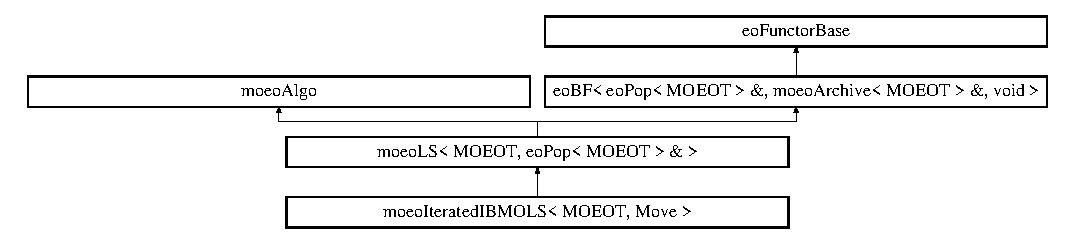
\includegraphics[height=3cm]{classmoeoIteratedIBMOLS}
\end{center}
\end{figure}
\subsection*{Public Types}
\begin{CompactItemize}
\item 
typedef MOEOT::Objective\-Vector \bf{Objective\-Vector}\label{classmoeoIteratedIBMOLS_bc0f8dff81be56b23376995aace92a01}

\begin{CompactList}\small\item\em The type of objective vector. \item\end{CompactList}\end{CompactItemize}
\subsection*{Public Member Functions}
\begin{CompactItemize}
\item 
\bf{moeo\-Iterated\-IBMOLS} (mo\-Move\-Init$<$ Move $>$ \&\_\-move\-Init, mo\-Next\-Move$<$ Move $>$ \&\_\-next\-Move, eo\-Eval\-Func$<$ MOEOT $>$ \&\_\-eval, \bf{moeo\-Move\-Incr\-Eval}$<$ Move $>$ \&\_\-move\-Incr\-Eval, \bf{moeo\-Binary\-Indicator\-Based\-Fitness\-Assignment}$<$ MOEOT $>$ \&\_\-fitness\-Assignment, eo\-Continue$<$ MOEOT $>$ \&\_\-continuator, eo\-Mon\-Op$<$ MOEOT $>$ \&\_\-mon\-Op, eo\-Mon\-Op$<$ MOEOT $>$ \&\_\-random\-Mon\-Op, unsigned int \_\-n\-Noise\-Iterations=1)
\begin{CompactList}\small\item\em Ctor. \item\end{CompactList}\item 
void \bf{operator()} (eo\-Pop$<$ MOEOT $>$ \&\_\-pop, \bf{moeo\-Archive}$<$ MOEOT $>$ \&\_\-arch)
\begin{CompactList}\small\item\em Apply the local search iteratively until the stopping criteria is met. \item\end{CompactList}\end{CompactItemize}
\subsection*{Private Member Functions}
\begin{CompactItemize}
\item 
void \bf{generate\-New\-Solutions} (eo\-Pop$<$ MOEOT $>$ \&\_\-pop, const \bf{moeo\-Archive}$<$ MOEOT $>$ \&\_\-arch)
\begin{CompactList}\small\item\em Creates new population randomly initialized and/or initialized from the archive \_\-arch. \item\end{CompactList}\end{CompactItemize}
\subsection*{Private Attributes}
\begin{CompactItemize}
\item 
\bf{moeo\-IBMOLS}$<$ MOEOT, Move $>$ \bf{ibmols}\label{classmoeoIteratedIBMOLS_6b1351f1faa391a1f095d1f9d4dba915}

\begin{CompactList}\small\item\em the local search to iterate \item\end{CompactList}\item 
eo\-Eval\-Func$<$ MOEOT $>$ \& \bf{eval}\label{classmoeoIteratedIBMOLS_7abdd0c1433ec4671522c8d5edc9fe61}

\begin{CompactList}\small\item\em the full evaluation \item\end{CompactList}\item 
eo\-Continue$<$ MOEOT $>$ \& \bf{continuator}\label{classmoeoIteratedIBMOLS_964e5df65c7aa33dd84eed3180d5e0a3}

\begin{CompactList}\small\item\em the stopping criteria \item\end{CompactList}\item 
eo\-Mon\-Op$<$ MOEOT $>$ \& \bf{mon\-Op}\label{classmoeoIteratedIBMOLS_77851daa2f2230000c0012beef3b8558}

\begin{CompactList}\small\item\em the monary operator \item\end{CompactList}\item 
eo\-Mon\-Op$<$ MOEOT $>$ \& \bf{random\-Mon\-Op}\label{classmoeoIteratedIBMOLS_89df3bfa7069c06c7e7cf4b30ccc5535}

\begin{CompactList}\small\item\em the random monary operator (or random initializer) \item\end{CompactList}\item 
unsigned int \bf{n\-Noise\-Iterations}\label{classmoeoIteratedIBMOLS_a50f25daf2847fb9d299ef65baf3bda7}

\begin{CompactList}\small\item\em the number of iterations to apply the random noise \item\end{CompactList}\end{CompactItemize}


\subsection{Detailed Description}
\subsubsection*{template$<$class MOEOT, class Move$>$ class moeo\-Iterated\-IBMOLS$<$ MOEOT, Move $>$}

Iterated version of IBMOLS as described in Basseur M., Burke K. 

: \char`\"{}Indicator-Based Multi-Objective Local Search\char`\"{} (2007). 



Definition at line 66 of file moeo\-Iterated\-IBMOLS.h.

\subsection{Constructor \& Destructor Documentation}
\index{moeoIteratedIBMOLS@{moeo\-Iterated\-IBMOLS}!moeoIteratedIBMOLS@{moeoIteratedIBMOLS}}
\index{moeoIteratedIBMOLS@{moeoIteratedIBMOLS}!moeoIteratedIBMOLS@{moeo\-Iterated\-IBMOLS}}
\subsubsection{\setlength{\rightskip}{0pt plus 5cm}template$<$class MOEOT, class Move$>$ \bf{moeo\-Iterated\-IBMOLS}$<$ MOEOT, Move $>$::\bf{moeo\-Iterated\-IBMOLS} (mo\-Move\-Init$<$ Move $>$ \& {\em \_\-move\-Init}, mo\-Next\-Move$<$ Move $>$ \& {\em \_\-next\-Move}, eo\-Eval\-Func$<$ MOEOT $>$ \& {\em \_\-eval}, \bf{moeo\-Move\-Incr\-Eval}$<$ Move $>$ \& {\em \_\-move\-Incr\-Eval}, \bf{moeo\-Binary\-Indicator\-Based\-Fitness\-Assignment}$<$ MOEOT $>$ \& {\em \_\-fitness\-Assignment}, eo\-Continue$<$ MOEOT $>$ \& {\em \_\-continuator}, eo\-Mon\-Op$<$ MOEOT $>$ \& {\em \_\-mon\-Op}, eo\-Mon\-Op$<$ MOEOT $>$ \& {\em \_\-random\-Mon\-Op}, unsigned int {\em \_\-n\-Noise\-Iterations} = {\tt 1})\hspace{0.3cm}{\tt  [inline]}}\label{classmoeoIteratedIBMOLS_67352bb5d797f20e767a4f0fa6d80f93}


Ctor. 

\begin{Desc}
\item[Parameters:]
\begin{description}
\item[{\em \_\-move\-Init}]the move initializer \item[{\em \_\-next\-Move}]the neighborhood explorer \item[{\em \_\-eval}]the full evaluation \item[{\em \_\-move\-Incr\-Eval}]the incremental evaluation \item[{\em \_\-fitness\-Assignment}]the fitness assignment strategy \item[{\em \_\-continuator}]the stopping criteria \item[{\em \_\-mon\-Op}]the monary operator \item[{\em \_\-random\-Mon\-Op}]the random monary operator (or random initializer) \item[{\em \_\-n\-Noise\-Iterations}]the number of iterations to apply the random noise \end{description}
\end{Desc}


Definition at line 86 of file moeo\-Iterated\-IBMOLS.h.

\subsection{Member Function Documentation}
\index{moeoIteratedIBMOLS@{moeo\-Iterated\-IBMOLS}!operator()@{operator()}}
\index{operator()@{operator()}!moeoIteratedIBMOLS@{moeo\-Iterated\-IBMOLS}}
\subsubsection{\setlength{\rightskip}{0pt plus 5cm}template$<$class MOEOT, class Move$>$ void \bf{moeo\-Iterated\-IBMOLS}$<$ MOEOT, Move $>$::operator() (eo\-Pop$<$ MOEOT $>$ \& {\em \_\-pop}, \bf{moeo\-Archive}$<$ MOEOT $>$ \& {\em \_\-arch})\hspace{0.3cm}{\tt  [inline]}}\label{classmoeoIteratedIBMOLS_52d4aa19a93c69ed0c2246c62821e76e}


Apply the local search iteratively until the stopping criteria is met. 

\begin{Desc}
\item[Parameters:]
\begin{description}
\item[{\em \_\-pop}]the initial population \item[{\em \_\-arch}]the (updated) archive \end{description}
\end{Desc}


Definition at line 111 of file moeo\-Iterated\-IBMOLS.h.

References moeo\-Iterated\-IBMOLS$<$ MOEOT, Move $>$::continuator, moeo\-Iterated\-IBMOLS$<$ MOEOT, Move $>$::generate\-New\-Solutions(), moeo\-Iterated\-IBMOLS$<$ MOEOT, Move $>$::ibmols, and moeo\-Archive$<$ MOEOT $>$::update().\index{moeoIteratedIBMOLS@{moeo\-Iterated\-IBMOLS}!generateNewSolutions@{generateNewSolutions}}
\index{generateNewSolutions@{generateNewSolutions}!moeoIteratedIBMOLS@{moeo\-Iterated\-IBMOLS}}
\subsubsection{\setlength{\rightskip}{0pt plus 5cm}template$<$class MOEOT, class Move$>$ void \bf{moeo\-Iterated\-IBMOLS}$<$ MOEOT, Move $>$::generate\-New\-Solutions (eo\-Pop$<$ MOEOT $>$ \& {\em \_\-pop}, const \bf{moeo\-Archive}$<$ MOEOT $>$ \& {\em \_\-arch})\hspace{0.3cm}{\tt  [inline, private]}}\label{classmoeoIteratedIBMOLS_2826cf283f6670b3c46da5ac6b6def18}


Creates new population randomly initialized and/or initialized from the archive \_\-arch. 

\begin{Desc}
\item[Parameters:]
\begin{description}
\item[{\em \_\-pop}]the output population \item[{\em \_\-arch}]the archive \end{description}
\end{Desc}


Definition at line 146 of file moeo\-Iterated\-IBMOLS.h.

References moeo\-Iterated\-IBMOLS$<$ MOEOT, Move $>$::eval, moeo\-Iterated\-IBMOLS$<$ MOEOT, Move $>$::mon\-Op, moeo\-Iterated\-IBMOLS$<$ MOEOT, Move $>$::n\-Noise\-Iterations, and moeo\-Iterated\-IBMOLS$<$ MOEOT, Move $>$::random\-Mon\-Op.

Referenced by moeo\-Iterated\-IBMOLS$<$ MOEOT, Move $>$::operator()().

The documentation for this class was generated from the following file:\begin{CompactItemize}
\item 
moeo\-Iterated\-IBMOLS.h\end{CompactItemize}
